\documentclass[a4paper]{article}

\usepackage[utf8]{inputenc}

\usepackage{url}
\usepackage[]{hyperref}

\usepackage{caption}

\usepackage{listings}

\usepackage{color}

% *** GRAPHICS RELATED packets ***
%\usepackage[pdftex]{graphicx}
\usepackage{graphicx}
%\usepackage[dvips]{graphicx}
% to place figures on a fixed position
\usepackage{float}

\usepackage[margin=1in]{geometry}


\lstdefinelanguage{Ini}
{
    basicstyle=\ttfamily\small,
    columns=fullflexible,
    morecomment=[s][\color{blue}\bfseries]{[}{]},
    morecomment=[l]{\#},
    morecomment=[l]{;},
    commentstyle=\color{gray}\ttfamily,
    morekeywords={},
    otherkeywords={=,:},
    keywordstyle={\color{green}\bfseries}
}


\title{Content Centric Networking (CCN) syllabus}
\author{}
\date{}


\begin{document}

\maketitle

\tableofcontents

\section{Introduction}

To be able to complete the Content Centric Networks laboratory, first you have to be familiar with
Mininet. Those who aren't, please study the \href{https://qosip.tmit.bme.hu/foswiki/pub/Meres/OpenFlowMSc/OpenFlow-Mininet-syllabus-en.pdf}{Mininet} laboratory instructions.

The IP protocol family, that is giving the technological base of the current Internet was and is 
constantly evolving. For example: at the first versions of the TCP protocol, the protocol running
 effectively on links with a then incredibly high, 10 Gbit/s speed wasn't an important aspect. The 
IP protocol family was constantly extended, so that it could support high degree mobility of endpoints,
 effective packet-transfer through erroneous links, and multiple-way data transfer among many others.
It was also an important aspect in planning, that the new versions could be constantly introduced,
i.e. the Internet could work even when only a part of the network devices and endpoints supported 
the new functions, that were currently introduced. This gradual evolution gave access to a continuous 
operation, in a way that the devices and software purchased and deployed earlier did not require to be
suddenly replaced, just because of the introduction of a new network function. But this also means,
that the planning decisions stated in the 1960's have an effect on today's technological environment
shaped by fundamentally different demands.

Facing the evolutionary planning model, that is granting continuous evolution, there is also the
clean slate planning model. The clean state model doesn't take the solutions designed in other
environments into consideration when designing a solution in the changed environment, hoping for
a more simple, clean and efficient solution. The content centric network (CCN) is also such an
experimental clean slate network protocol, that is able to work above IP. Moreover, CCN networks
are able to transfer IP packets in principle. This way, it is a clean slate network, at the 
implementation of which there was a lot of attention paid to the opportunity of gradual introduction.

But what is the point to get to know such an experiment protocol, if it is not likely, that we will 
see them in real systems in the near future? In a paradoxical way, getting to know a system that is 
completely different from the current Internet can draw attention to the solutions that we take for
granted, or about which we think, couldn't be done in a different way. For example, in the 1960's 
the creation of computer-networks was motivated by the sharing of the exceptionally expensive 
resources. The IP protocol was built upon the communication of a peer sharing and a different peer
using the resources. That is why the IP-addresses of both the source host and the destination 
host can be seen in the IP packets. The IP-address identifies the device itself, so creating a 
multi-cast traffic where a packet can have multiple destinations is rather complex. But since the
60's the main function of networks has been gradually changing from resource-sharing to content-
sharing. Back then the important thing was to find the given "high-speed" magnetic tape data reader
or the supercomputer with a high computing capacity. But when browsing the web, the exact location
of a html file is not important, but rather the content of the file. In more detail: the priority is
for the users browser to be able to display the html page (stored in multiple places for
security-related reasons) as soon as possible. Using multi-cast, peer-to-peer, or Content Delivery Network (CDN) networks over
IP is also possible, but these would demand additional network protocols, application-level solutions,
or additional network nodes. To these tasks, CCN grants a much more natural and clear solution.

\begin{figure}[H]
    \centering
    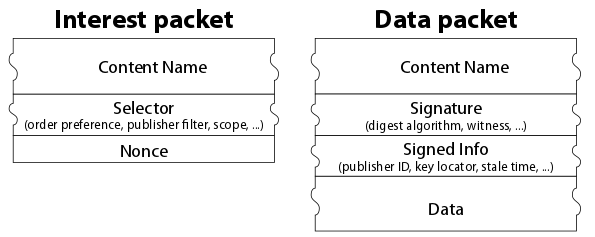
\includegraphics[width=0.9\textwidth]{figures/ccn-packets.png}
    \caption{CCN packet-types~\cite{CongestionAvoidance}}
    \label{fig:CCN-packet-types}
\end{figure}


In the case of CCN we differentiate between two types of packets: the ones requesting data (interest)
and the ones with actual content. As also seen in Figure~\ref{fig:CCN-packet-types}, the packets don't only contain the 
addresses of the source host and the destination host, but also a name clearly represent the
content itself. This content-name - similarly to the IP-address - is built up hierarchically.
The interest packets are sent into the network by the entity that is requesting data. Then the network 
gets the request to the source host, but the route of the packet is remembered by the nodes 
forwarding it. The data source answers the request with a data packet, which takes the exact 
same route to the requesting host. Many details of this process are not yet clarified, but we
can already clearly see two differences in comparison to the TCP/IP system:
\begin{enumerate}
\item There is no acknowledgment arriving to the data packets, but there is one arriving for the
interest packet, that can be seen as some kind of acknowledgment of the interest.
\item In  contrast to the TCP/IP system, it is guaranteed, that the route consists of the same
nodes in the case of the request packet as in the case of the data packet.
\end{enumerate}

\begin{figure}[H]
    \centering
    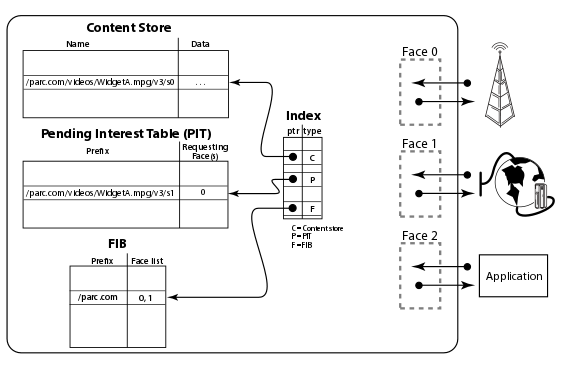
\includegraphics[width=0.9\textwidth]{figures/ccn-node.png}
    \caption{CCN forwarding nodes sketch~\cite{CongestionAvoidance}}
    \label{fig:CCN-nodes}
\end{figure}


The rough sketch of the node responsible for forwarding packets can be seen on Figure~\ref{fig:CCN-nodes}. The node
communicates with other nodes and applications through so-called faces, instead of interfaces used
in IP. It is crucial to see that the node contacts sources and interests on the same API, as it does
with other nodes, since from the perspective of the node, the application is just a communicating
half, that subscribes only to a particular content-prefix.

If an arriving interest can be found in the Content Store, then the node creates a packet with the
data found in the Content Store, sends it as an answer in the direction of the request, then throws
the request away. If the request cannot be satisfied with the data found in the Content Store, it 
gets included in the Pending Interest Table (PIT). The table contains the following data: which name
prefixes have been requested, and from where. Then, if there has been a log completely identical to
the given prefix in the node, the request gets thrown away. If this is the first time, that this 
request can be found in the PIT, the name of the request and the face it arrived from, also gets
included. If this is the first time, that this request can be found in the PIT, the Forwarding 
Information Base (FIB) decides, what happens to the packet. The node looks for the name of the 
request by looking for longest parity at the beginning of each word. In case of finding it, the node
sends the request to the faces belonging to the prefix, leaving out the face that sent the request.

One can see that the queues causing difficulties in setting up IP networks are completely 
missing from the nodes. The data gets included into the Content Store, but it only has a role in 
satisfying latter requests early. The capacity of the Content Store is finite, if it gets full, the
element used the longest ago gets thrown away, by default.

The Content store gives access to very efficient multi-transfer. In the case of multi-transfer,
the requesting hosts all want the same content, so they all send the same request. If two requests
follow each other within a small amount of time, then two faces get included beside the request into
the PIT of the CCN node. On the other hand, if the node already attended the first request, the 
second one can be satisfied with the data from the Content Store. In both cases, the node that got 
the two requests, forwards the request in the direction of the data source only once, and they send
the content to the node only once. What's more, data transfer doesn't need to be delayed because of
any kind of multi-transfer group-building protocol. 

A data packet always gets back to the requesting host on the same route. However, there can be 
multiple faces in the same FIB log, so the request-packet gets forwarded on multiple faces, and this
can be useful, if the appropriate content can be found in multiple places. (The cycles occurring
because of this can be detected with the help of the Nonce field of the request-packet. This field
got removed from the newer versions of CCN, and cycle-detection got solved in another way.
Furthermore, there is also an opportunity - with the specific settings - that the node forwards the
request-packet to only one of the faces.)

In the case of IP, defense against interception and data-falsification can be done by encrypting the
channel, or ensuring its integrity. In the case of CCN, instead of the channel, we protect the
data itself. The forwarding nodes can fit the hierarchic content-name out with their digital 
signatures in diversely deep ways. What's more, any forwarding node can check the authenticity of the
content, because CCN uses an encryption with a public key. That's why certain overflow attacks can be
stopped inside the network, and detecting the attack isn't the job of only the requesting host (as 
it is in the case of IP). Take the content name /parc.com/george/videos/WidgetA.mpg as an example.
The video-file doesn't fit into one single data-packet, so it gets segmented by the sender. The name
of the request doesn't contain the ordinal number of the segment, so the response will contain the
first segment with the following content name: /parc.com/george/videos/WidgetA.mpg/s0 . The George
user can authenticate the data-packet with his own key, that was authenticated by parc. The 
authentication chain produces a distributed authentication netwotk without a central entity. (The 
second part of the video can be requested from the name /parc.com/george/videos/WidgetA.mpg/s1 .)


\bibliographystyle{unsrt}
\bibliography{references}

\appendix

\section{Lab exercises}


\subsection{Lab report}

Please create and send a lab report as instructed by the lab demonstrator. For taking screen-shots, you can use the \verb!xfce4-screenshooter! application, but it is 
recommended to copy-paste the output of the terminal window into the report, because this way it is
easier to highlight the more harsh parts. You can use \verb!draw.io! to create nice network topologies.


\subsection{Task: Getting familiar with mini-ccnx}
`
There are many versions of CCN, some of these have multiple prototypes. The ccnx prototype was 
designed by the Xerox Parc Research Center, under the direction of Van Jacobson. Later, he continued
his work individually of the Parc, in the Named Data Networking project. Different implementations 
have different abilities and contain different errors. Over the course of the laboratory session, 
we are going to use an old implementation by parc, ccnx 0.8.2. Instead of real instruments, we are
going to use the packet-forwarding engine and the different support programs of ccnx in a Mininet
environment. Mini-ccnx is a modification of Mininet, that beside virtualizing end points and 
laying out network topology, also starts and configures CCN programs. Unlike Mininet, mini-ccnx
starts the network based on a configuration file in 'ini' format. The official syllabus to using the
file is relatively easy to understand, but contains some basic mistakes:
\url{https://github.com/chesteve/mn-ccnx/wiki/Tutorial}

\begin{itemize}

\item The order of the items must be: [preferences], [routers], [hosts], [links]. There is no 
such item as [nodes]. The syntax of the item [hosts] is identical to the one described for [nodes].
The [routers] part is almost identical to the [nodes] part, but the application doesn't need to be 
given, so after the name come the forwarding rules.
\item The item [preferences] can be produced with the \verb!miniccnxedit! command, but the command
cannot really be used for anything else. Here's an example:

\begin{lstlisting}[language=Ini,breaklines]
[preferences]
getMetrics: 1
ipBase: 10.0.0.0/8
startCLI: 1
dbPort: 8086
dbHost: localhost
dbPass: root
dbName: miniccnx_data
dbUser: root
terminalType: xterm
metricsTimer: 30.0
templatePath: miniccnx.conf
\end{lstlisting}

\item If we don't want to start an application automatically to a host in the item [hosts], but
we want to give forwarding rules, we need to put an underscore character between single quotation
marks:
\begin{lstlisting}[language=Ini,breaklines]
   h1: '_' ccnx:/,s1
\end{lstlisting}

\end{itemize}

The task is to create a h1-s1-h2 network seen in the tutorial with the forwarding rules seen there! Run the
\verb!ccndump mininet! command, and interpret its output!

\subsection{Task: Two node network, ccnping}

Let's look at the round-trip time between h1 and h2 using the commands \verb!ccnping! and \verb!ccnpingserver!.
If necessary, modify the \verb!miniccnx.conf! file, so the system can start with the appropriate routing logs.

Compare the outputs of the \verb!ccndstatus! program with h1,s1,h2 computers, before, during and after running
the \verb!ping! commands. How can the new, modified or missing entries explained? (The entries that didn't
change during running the command, don't need to be fully understood.)

Modify the configuration file in a way that the \verb!pingserver! automatically starts when mini-ccnx does.
In other words, name an application that starts automatically. (Mini-ccnx doesn't continue the 
initialization until the applications belonging to the hosts stop running, so the \verb!pingserver! has to
be started in the background: it is a good decision to put an \& character after the command line.)

\subsection{Task: Examining mobility with the commands: ping, linkdown}

\begin{figure}[H]
    \centering
    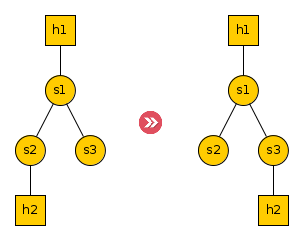
\includegraphics[width=0.9\textwidth]{figures/unnamed0.png}
    \caption{Topology for evaluating network mobility. The delay on each link is 10ms.}
    \label{fig:CCN-topo}
\end{figure}

In this task we investigate the effect mobility has on ccn traffic. The goal is for the h2 connected
to the \verb!pingserver! running on h1 - similarly to Figure~\ref{fig:CCN-topo} - to reach h1 through different nodes after
some time. Unfortunately, mini-ccnx doesn't support moving nodes. That's why the best option is to
connect h2 to s2 through s4. S4 should also be connected to s3. Then, we can produce the configuration
seen in Figure~\ref{fig:CCN-topo} using \verb!mininet!'s link command. It isn't pretty, but it does the job.

\subsection{Task: Investigating multi-transfer with the commands ccnpeek and ccnpoke}

Let's look at the way these commands work. Create a \verb!mininet! topology, through which we can show that
in the case of multi-transfer, the network doesn't send packets of no use. Let's show what happens
when a destination host already received the requested content when the other destination host sends
its request into the network. Let's also check what happens if the second request comes before the
first one gets a response from the source.

\end{document}